\documentclass[12pt]{article}
\usepackage{amsmath}
\usepackage[lmargin = 0.2in, rmargin = 0.2in, tmargin = 0.1in, bmargin = 0.5in]{geometry}
\usepackage[none]{hyphenat}
\usepackage{graphicx}
\usepackage{subcaption}

\title{\textbf{Assignment 4 Bonus}}
\author{Aditya Vipradas\\ASU ID: 1209435588}
\begin{document}
\maketitle

The given function is $f(x) = cos x$ which can be written in the polynomial form using Taylor Series as,
\begin{equation}
cos(x) = 1 - \frac{x^{2}}{2!} + \frac{x^{4}}{4!} - \frac{x^{6}}{6!} + \frac{x^{8}}{8!} - ...
\end{equation}
The number of gauss quadrature points are determined from the order of the polynomial equation being used. The relation between the integration points ($n_{gp}$) and the order of the polynomial ($p$) is determined from the following equation.
\begin{equation}
n_{gp} >= \frac{p+1}{2}
\end{equation}
Thus, the more the number of integration points, the more the polynomial order it can integrate. Let us approximate the $f(x) = cos x$ function up to $6^{th}$ order so that 4 point gauss quadrature can be used. The rate of convergence can now be determined using the equation as shown below.
\begin{equation}
log(||e||_{L2}) = C + (\alpha)log(h)
\end{equation}
Here, the rate of convergence is nothing but the slope ($\alpha$) of the line plot of $log(||e||_{L2})$ vs $log(h)$. $C$ is the y-intercept of this line. This line plot can be obtained by reducing the element length size ($h$) and calculating the corresponding L2 norm of the displacement ($e1$) and strain ($e2$) errors. The log-log plot of all the L2 norms of the errors corresponding to the respective element length sizes can then be plotted. In this case, element size is reduced by increasing the number of nodes gradually in the given interval. To start with, 10 nodes are considered and they are incremented by 5 up to 1000 nodes. A 4-point gauss quadrature is used. The following plots are obtained.

\begin{figure}[ht]
\begin{center}
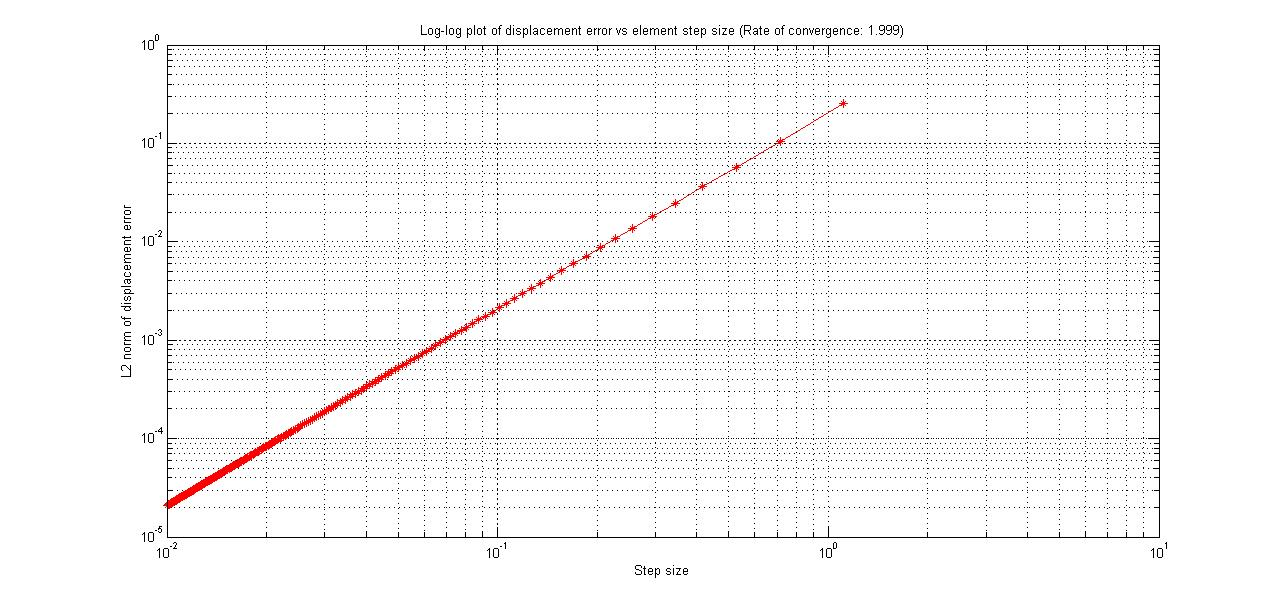
\includegraphics[scale=0.4]{disp.jpg}
\end{center}
\end{figure}
As observed from this plot, the slope or rate of convergence for the displacement error ($e1$) when two-node linear elements are used is 1.999.
And as seen from the following plot, the slope or rate of convergence for the strain error ($e2$) when two-node linear elements are used is 0.999.\\
\begin{figure}[ht]
\begin{center}
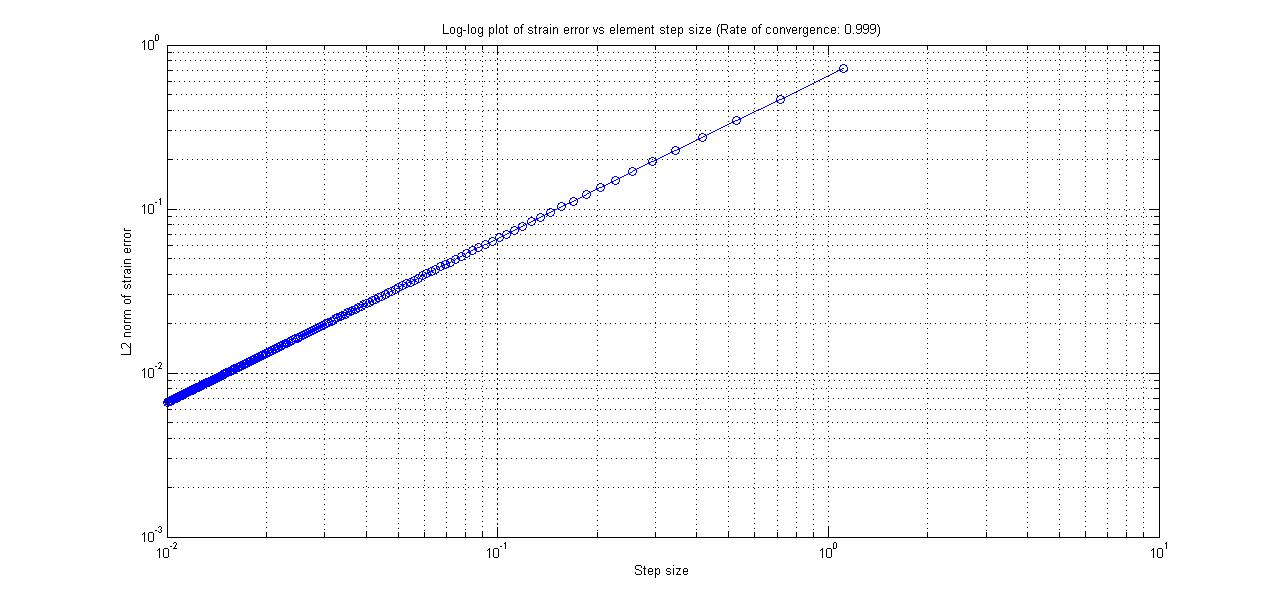
\includegraphics[scale=0.35]{strain.jpg}
\end{center}
\end{figure} 
 
When the total number of nodes is raised to 2000, the rates of convergence for displacement ($e1$) and strain ($e2$) errors are 1.999 and 1.000 respectively which are in agreement to values obtained previously. Hence, these values are acceptable. This represents that if the element size reduces by $z$, the displacement and strain errors reduce by $z^{2}$ and $z$ respectively. This is the procedure to determine the converge rates of the given elements.
\end{document}